\documentclass[12pt]{article}

\usepackage{color}
\usepackage[english]{babel}
\usepackage[utf8]{inputenc}
\usepackage{indentfirst}
\usepackage{graphicx}
\usepackage{verbatim}
\usepackage{listings}
\usepackage{url}
\usepackage{stringenc}
\usepackage{pdfescape}
\usepackage{subfig}
\usepackage{float}
\usepackage{csquotes}  

\usepackage[toc,page]{appendix}

\begin{document}

\setlength{\textwidth}{16cm}
\setlength{\textheight}{22cm}
\title{\huge{\textbf{\textit{aWareHouse}}}\linebreak
\Large\textbf{\\Environment Control System for Warehouses}\linebreak\linebreak\linebreak

\includegraphics[width=8cm]{feup.pdf}\linebreak \linebreak
\large{MSc in Informatics and Computer Engineering} \linebreak
\large{Programming Paradigms \\ EIC0065-2S}\linebreak
}
\author{
Duarte Nuno Pereira Duarte - 201109179 (ei11101@fe.up.pt)\\
Hugo José Freixo Rodrigues - 201108059 (ei11086@fe.up.pt)\\
João Pedro Matos Teixeira Dias - 201106781 (ei11137@fe.up.pt)\\
\\
\\ Faculdade de Engenharia da Universidade do Porto \\ Rua Roberto Frias, s\/n, 4200-465 Porto, Portugal
 \vspace{1cm}}
%\date{Junho de 2007}
\maketitle
\thispagestyle{empty}

%************************************************************************************************
%************************************************************************************************

\newpage
\section*{Abstract}

We are in the rise of IoT (Internet of things). A world were everything is connected and we can, with simple tools, monitory and control everything. In this context, there is a lot of space for a more recurrent use of different programming paradigms because of the need of interaction with different layers of system architecture for a single application, since hardware to web.

Our application, \textit{aWareHouse}, was designed with the objective of, with a simple interface, we can monitory a house or a warehouse in terms of environment conditions (temperature, humidity, sound and luminosity). 

For accomplishing this was used a combination of hardware/software and some different programming languages, in a way that gave us a stable application that can be used for setting a alarm system when occurs changes in our environment, for taking decisions analysing the past conditions and the relations with external (meteorological) conditions or simple look at the current conditions inside our warehouse.


\newpage
%************************************************************************************************
%************************************************************************************************
\tableofcontents
%************************************************************************************************
%************************************************************************************************
\newpage

\section{Introduction}

The \textit{aWareHouse} project was developed for the Programming Paradigms course unit of the Master in Informatics and Computing Engineering at FEUP. The project was developed with the objective of combine, at least, three programming paradigms in the same application.

The base motivation for this project was the Internet of Things, as defined by \textit{Gartner}:

\blockquote{The Internet of Things (IoT) is the network of physical objects that contain embedded technology to communicate and sense or interact with their internal states or the external environment.}

So, we designed a low cost system capable of giving the user the possibility of, using a relative small hardware box, monitory the environment of a given place like a home or warehouse. This, associated with a system capable of maintain records of the past conditions of the environment (plus external weather conditions), results in one application that gives the user the capacity of taking decision, be aware of the environment status using alerts and see the current conditions.

As explained before the capabilities of this application make this a system useful in a lot of situations, for example, the monitoring of a warehouse and verify the relation between weather and internal conditions to make decision on what is the best settings for a refrigeration system and assure that the, for example, temperature is always below the maximum recommended. Other example is simple use it as a house control system and, for example, verify if someone forgot to turn any light off.

\newpage
\section{System Description}
\subsection{Conceptual Description}
\subsubsection{Functionalities}
\begin{figure}[h]
    \centering
    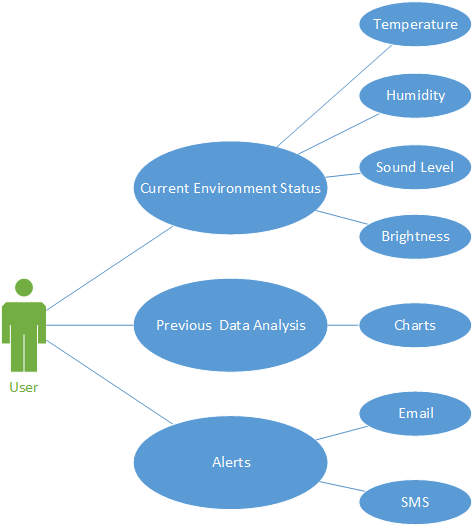
\includegraphics[scale=0.7]{use.png}
    \caption{Use Case diagram.}
    \label{fig:use}
\end{figure}

\subsubsection{Architecture}
\begin{figure}[h]
    \centering
    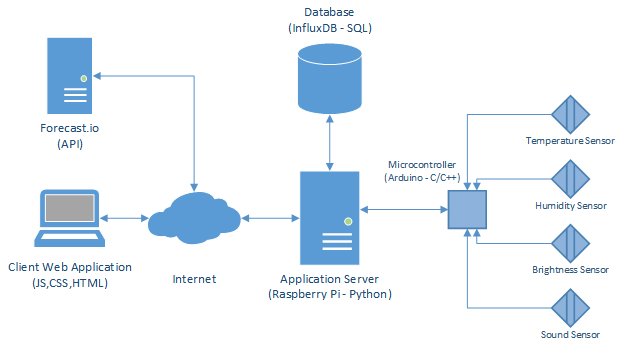
\includegraphics[scale=0.85]{arc.png}
    \caption{Architecture diagram.}
    \label{fig:use}
\end{figure}

\subsubsection{Programming Languages and Technologies}
\subsection{Implementation Description}
\subsubsection{Implementation Details}
\subsubsection{Development Environment}
\newpage
\section{Conclusion}
\newpage
\section{Improvements}
\newpage
\section{Resources}
\subsection{\it{Bibliography}}
\begin{description}
\item Visual Studio 2013 Ultimate, Microsoft, \url{http://www.visualstudio.com/}.
\end{description}
\subsection{\it{Software}}
\begin{description}
\item Visual Studio 2013 Ultimate, Microsoft, \url{http://www.visualstudio.com/}.
\end{description}

\newpage

\begin{appendices}
\section{Appendix}
The contents...
\end{appendices}

\end{document}
